% !TeX spellcheck = it_IT
\newpage
\section{Equazioni non lineari}
Stiamo considerando equazioni del tipo $f(x)=0$ dove la funzione $f$ non è lineare (quindi non è una retta). Di fronte a questo tipo di equazioni, ci sono due difficoltà:
\begin{itemize}
	\item Non c'è una teoria generale sul \textit{numero} e sull'\textit{esistenza} delle \textbf{soluzioni}
	\item Non esistono metodi diretti di risoluzione
\end{itemize}

\begin{example}
	Determinare il numero di soluzioni reali dell'equazione
	\begin{equation*}
		f(x)=x \log x -1 = 0
	\end{equation*}
	Il primo passo è tracciare un grafico approssimativo di questa funzione:
	\begin{itemize}
		\item \textbf{Dominio}: $x>0$
		\item \textbf{Limiti}:
		\begin{align*}
			& \lim_{x \to + \infty} x \log x -1 = + \infty \\
			& \lim_{x \to 0^+} x \log x = \lim_{x \to 0^+} \frac{log x}{\frac{1}{x}} = \lim_{x \to 0^+} \frac{\frac{1}{x}}{-\frac{1}{x^2}} = \lim_{x \to 0^+} - \frac{x^2}{x} = 0 \Longrightarrow \lim_{x \to 0^+} x log x -1 = -1 
		\end{align*}
		\item \textbf{Derivata prima}: \begin{align*}
			& f'(x) = \log x + x \cdot \frac{1}{x} = \log x + 1 \\
			& f'(x) \geq 0 \Leftrightarrow log x + 1 \geq 0 \Leftrightarrow log x \geq -1 \Leftrightarrow x \geq \frac{1}{e}
		\end{align*}
		\item \textbf{Derivata seconda}: $f''(x)=\frac{1}{x} \geq 0 \quad \forall x > 0$
	\end{itemize}
	\begin{center}
		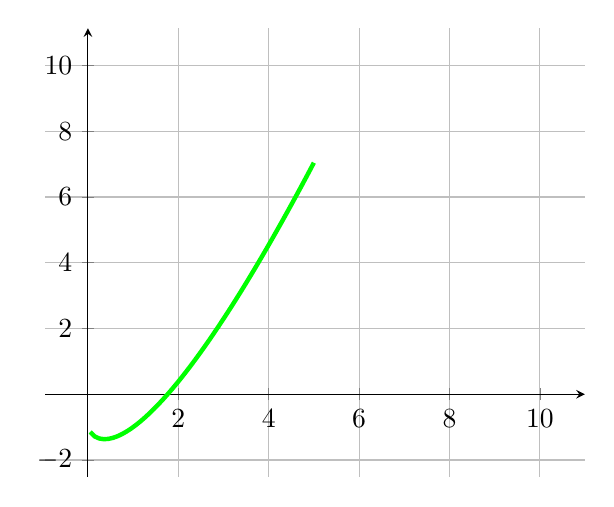
\begin{tikzpicture}
			\begin{axis}[grid=both,
				xmax=10,ymax=10,
				axis lines=middle,
				samples=100,
				enlargelimits]
				\addplot[green, ultra thick]  {x*ln(x)-1};
			\end{axis}
		\end{tikzpicture}
	\end{center}
	Quindi possiamo dire che 
	\begin{equation*}
		\exists ! \alpha \in \mathbb{R} \vert f(\alpha) = 0
	\end{equation*}
	Ci serve dare un \textbf{intervallo di localizzazione} della soluzione, ad esempio:
	\begin{align*}
		& f(1) = -1 \\
		& f(2) = 2 \log 2 -1 = log 4 -1 \\
		& \Rightarrow \alpha \in [1,2]
	\end{align*}
\end{example}

\subsection{Tecnica della separazione}
A partire da una funzione complessa, mi riconduco a funzioni più semplici e vedo dove si intercettano.
\begin{example}
	Supponiamo di avere
	\begin{equation*}
		x \log x -1 = 0 \Leftrightarrow x \log x = 1 \Leftrightarrow \log x = \frac{1}{x}
	\end{equation*}
	Che sul grafico sono
	\begin{center}
		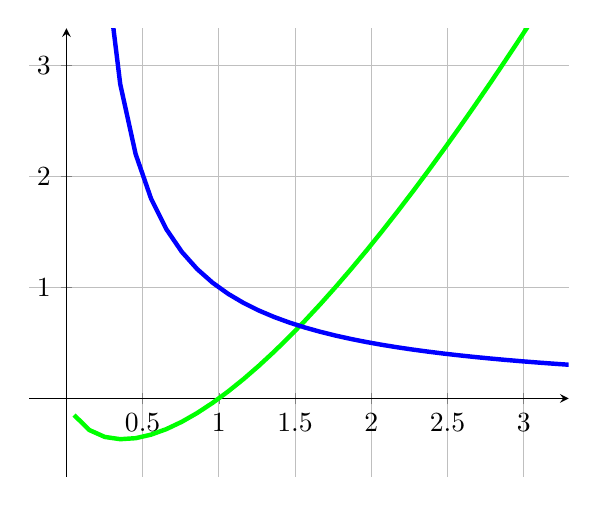
\begin{tikzpicture}
			\begin{axis}[grid=both,
				xmax=3,ymax=3,
				axis lines=middle,
				restrict x to domain=0:4,
				restrict y to domain=-2:4,
				samples=100,
				enlargelimits]
				\addplot[green, ultra thick]  {x*ln(x)};
				\addplot [blue, ultra thick] {1/x};
			\end{axis}
		\end{tikzpicture}
	\end{center}
\end{example}

\begin{example}
	Data la seguente funzione
	\begin{equation*}
		f(x) = e^x - 2x = 0 \Leftrightarrow e^x = 2x
	\end{equation*}
	È difficile usare il metodo della separazione perché l'intersezione non è facile da trovare. \\
	Usiamo quindi la soluzione grafica:
	\begin{itemize}
		\item \textbf{Dominio}: $\forall x \in \mathbb{R}$ che possiamo scrivere anche come $C^\infty (\mathbb{R})$
		\item \textbf{Limiti}:
		\begin{align*}
			& \lim_{x \to + \infty} e^x -2x = \lim_{x \to + \infty} e^x (1 - \frac{2x}{e^x}) = 0\\
			& \lim_{x \to - \infty} e^x -2x = + \infty\\
		\end{align*}
		\item \textbf{Derivata prima}: \begin{align*}
			& f'(x) = e^x -2 \\
			& f'(x) \geq 0 \Leftrightarrow e^x \geq 2 \Leftrightarrow x \geq \log 2
		\end{align*}
		\item \textbf{Derivata seconda}: $f''(x)=e^x$
	\end{itemize}
	\begin{center}
		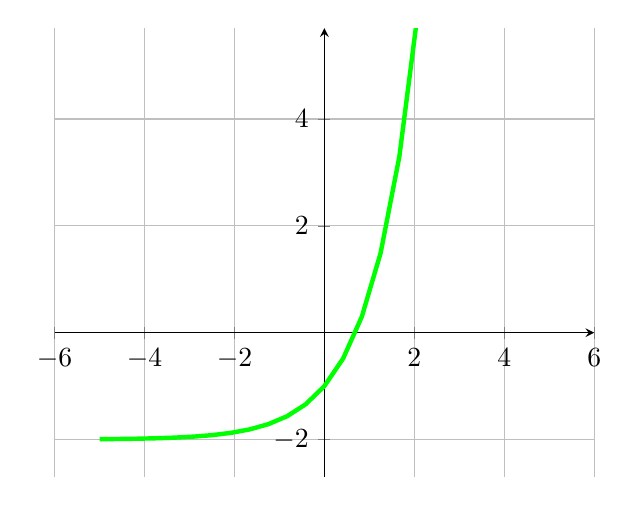
\begin{tikzpicture}
			\begin{axis}[grid=both,
				xmax=5,ymax=5,
				axis lines=middle,
				enlargelimits]
				\addplot[green, ultra thick]  {pow(e,x)-2};
			\end{axis}
		\end{tikzpicture}
	\end{center}	
	Calcoliamo adesso il valore in $\log 2$:
	\begin{equation*}
		f(\log 2) = e^{\log 2} - 2 \log 2 = 2-2 \log 2 = 2 (1-\log 2)
	\end{equation*}
\end{example}

\begin{example}
	Data la funzione:
	\begin{equation}
		f(x)= x^3 -6x +1 = 0
	\end{equation}
	In questo esempio abbiamo un polinomio e abbiamo quindi un'\textbf{equazione algebrica} di terzo grado. Quindi sappiamo il numero di soluzioni \textit{complesse}, nel nostro caso $3$. A noi però interessa il numero di soluzioni reali. Sapendo che quelle complesse devono andare sempre in coppia, potremo avere o due soluzioni complesse e una reale oppure tre soluzioni reali. Studiamo la funzione:
	\begin{itemize}
		\item \textbf{Dominio}: $\forall x \in \mathbb{R}$
		\item \textbf{Limiti}:
		\begin{align*}
			& \lim_{x \to + \infty} x^3 -6x +1 = + \infty\\
			& \lim_{x \to - \infty} x^3 -6x +1 = - \infty\\
		\end{align*}
		Sappiamo quindi che esiste sicuramente almeno un punto in cui la funzione vale $0$ per il teorema dell'esistenza degli zeri.
		\item \textbf{Derivata prima}: \begin{align*}
			& f'(x) = 3x^2-6 \\
			& f'(x) = 0 \Leftrightarrow x^2 = 2 \Leftrightarrow x = \pm \sqrt{2} \to x < -\sqrt{2} \land x > \sqrt{2}
		\end{align*}
		\item \textbf{Derivata seconda}: $f''(x)=6x \to f''(x) > 0 \Leftrightarrow x>0$
	\end{itemize}
	\begin{center}
		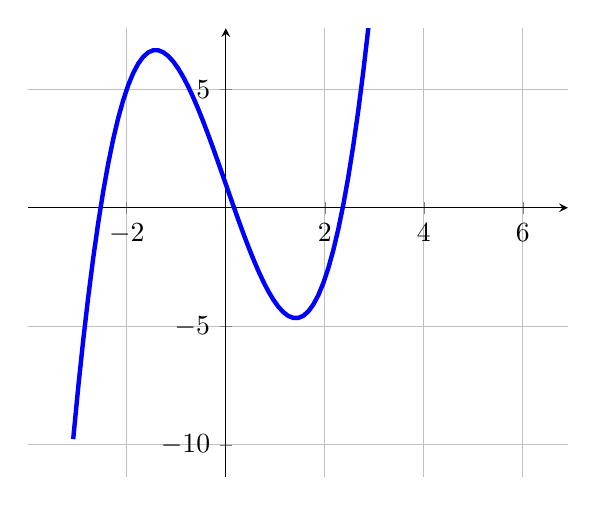
\begin{tikzpicture}
			\begin{axis}[grid=both,
				xmax=6,ymax=6,
				axis lines=middle,
				restrict x to domain=-4:4,
				restrict y to domain=-10:10,
				samples=100,
				enlargelimits]
				\addplot[blue, ultra thick] (x,x^3-6*x+1);
			\end{axis}
		\end{tikzpicture}
	\end{center}
	Quindi ci sono tre soluzioni reali, che possiamo localizzare come:
	\begin{align*}
		& \beta \in [0, \sqrt{2}]\\
		& \gamma \in [\sqrt{2}, 3]\\
		& \alpha \in [-3,-2]
	\end{align*}
\end{example}
\newpage
\subsection{Metodo di bisezione}
Vogliamo risolvere un'equazione $f(x)=0 \quad f:[a,b]\to \mathbb{R}$ che assumiamo essere \textit{continua} ($f \in C^0([a,b])$). Supponiamo poi che $f(a)f(b) < 0$, quindi la funzione assume valori discordi agli estremi. Questo implica, grazie al teorema di esistenza degli zeri, che $\exists \alpha \in [a,b] \:\vert f(\alpha)=0$, ovvero che esiste almeno un punto di intersezione con l'asse delle x.\\
Assumiamo che esista unico il punto di intersezione:
\begin{equation*}
	\exists ! \alpha \in [a,b] \:\vert\: f(x)=0
\end{equation*}
In questa situazione possiamo costruire diverse successioni che convergono ad $\alpha$ tramite il metodo di bisezione.
\begin{lstlisting}[language=MatLAB]
	a0 = a; b0=b; ya=f(a); yb=f(b);
	for k=1 : inf
		Ck = (a[k-1] + b[k-1])/2; % Calcolo il punto di mezzo dell'intervallo
		y = f(Ck);
		if(y * ya <= 0)
			ak = a[k-1]; bk=Ck; yb=y; % Qui la funzione e' discorde, mi sposto su questo intervallo
		else
			ak=Ck; bk=b[k-1]; ya=y; % Qui e' concorde, mi sposto sull'altro intervallo
		end
	end
\end{lstlisting}
Praticamente prendo il punto medio e controllo quale parte della funzione è concorde o discorde e mi sposto di conseguenza.
\begin{observation}
	Possiamo fare le seguenti osservazioni:
	\begin{enumerate}
		\item $a_k \leq b_k \quad \forall k$
		\item $\alpha \in [a_k, b_k] \quad \forall k$
		\item $b_k - a_k = \frac{b_{k-1}-a_{k-1}}{2} = \ldots = \frac{b_0 - a_0}{2^k}$
	\end{enumerate}
	che implicano:
	\begin{align*}
		& 0 \leq \lvert \alpha - a_k \rvert \leq b_k - a_k = \frac{b_0 - a_0}{2^k}\\
		& 0 \leq \lvert \alpha - b_k \rvert \leq b_k - a_k = \frac{b_0 - a_0}{2^k}\\
		& 0 \leq \lvert C_k  - \alpha \rvert \leq b_{k-1} - a_{k-1}\leq= \frac{b_0 - a_0}{2^k}
	\end{align*}
	e portando $k$ all'infinito, $a_k$, $b_k$ e $C_k$ tendono tutti ad $\alpha$.
\end{observation}

\begin{example}
	Supponiamo di voler risolvere
	\begin{equation*}
		f(x)=x-\cos x = 0
	\end{equation*}
	\newpage
	Proviamo prima con la \textbf{tecnica della separazione}:
	\begin{center}
		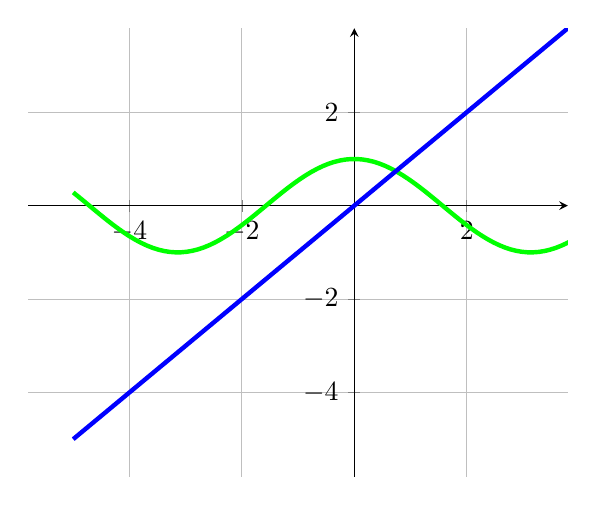
\begin{tikzpicture}
			\begin{axis}[grid=both,
				xmax=3,ymax=3,
				axis lines=middle,
				restrict x to domain=-5:5,
				restrict y to domain=-5:5,
				samples=100,
				enlargelimits]
				\addplot[green, ultra thick]  {cos(deg(x))};
				\addplot [blue, ultra thick] {x};
			\end{axis}
		\end{tikzpicture}
	\end{center}
	Osservando  attentamente notiamo che
	\begin{equation*}
		\exists ! \alpha \in [0,1]
	\end{equation*}
	poiché fuori da questo intervallo la funzione $x$ assume valori maggiori di $1$ o minori di $-1$ che non sono valori che può assumere la funzione $cos(x)$.\\
	Per poter usare il \textbf{metodo della bisezione} devo verificare che $f(x)$ sia continua e la sua monotonia.\\
	Come estremi per il metodo possiamo porre $[a,b]=[0,1]$.
	\begin{equation*}
		\lvert C_k - \alpha \rvert \leq \frac{b_0 - a_0}{2^k} \leq \epsilon
	\end{equation*}
	Posso a priori decidere la distanza dal mio numero finale facendo $\log_2 \frac{1}{\epsilon}$ passi.
\end{example}

\subsubsection{Approssimazione della radice}
Supponiamo di voler risolvere
\begin{equation*}
	x^2-2=0
\end{equation*}
Sappiamo che le soluzioni sono $x=\pm \sqrt{2}$ e che il grafico è:
\begin{center}
	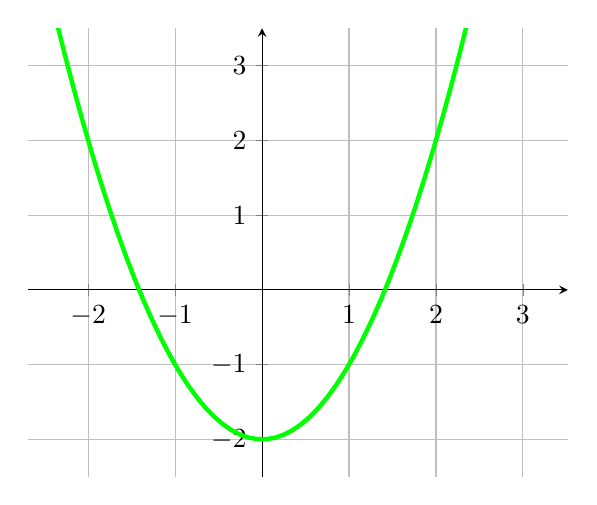
\begin{tikzpicture}
		\begin{axis}[grid=both,
			xmax=3,ymax=3,
			axis lines=middle,
			restrict x to domain=-5:5,
			restrict y to domain=-5:5,
			samples=100,
			enlargelimits]
			\addplot[green, ultra thick]  {x^2-2};
		\end{axis}
	\end{tikzpicture}
\end{center}
Il calcolatore non sa come calcolare $\sqrt{2}$, il modo migliore per farglielo fare è approssimare questa funzione con il metodo di bisezione nell'intervallo $[0,2]$.

\subsubsection{Svantaggi}
Questo metodo ha fondamentalmente due svantaggi:
\begin{itemize}
	\item Ha difficoltà ad essere esteso ai numeri \textbf{complessi}, ma per il nostro corso non ci riguarda
	\item Il \textbf{costo computazionale} è molto influenzato dal numero di valutazioni della funzioni che faccio e, dato che non conosco precisamente quali calcoli dovrà fare, potrebbe essere un problema. Nel metodo di bisezioni faccio una valutazione per passo e il numero di passi potrebbe essere elevato.
\end{itemize} 